\chapter{Distributed Data Aggregation}
\section{Definition}
Data aggregation is a technique that consists, on its basis, in reduce the amount of data collected, reducing the resources needed to process it.  According to \cite{journals/corr/abs-1110-0725}, data aggregation is  considered a subset of information fusion, that aims at reducing the handled data volume. A more precise definition is given in the same report:
\begin{definition} An aggregation function $f$ takes a multiset of elements from a domain $I$ and produces an output of a domain $O$.
\begin{equation*} f : \mathbb{N}^I \to O \end{equation*}
\end{definition}
The order in which the elements are aggregated is irrelevant and a given value may occur several times. As the main goal of data aggregation, the aggregation function aims to summarize information. The result of an aggregation takes less space than the inputed multiset (element from $\mathbb{N}^I$).\\
Distributed data Aggregation or \textit{in-network} aggregation means that it is a task which is distributed among several nodes in the network. In contrary of a \textit{centralized} arquitecture, where a central node compute all the data and performs the aggregation function, a \textit{de-centralized} aggregation distribute the data, hence the effort to compute the aggregation function is reduced.
\subsection {Decomposable functions}
\todo{Correct definition? Need to specify more why decomposable functions could be computed in a parallel or distributed way}
For some aggregation function, one node may need to perform a single computation operation involving all the elements of the multiset, requiring more resources than the ideal ones. So, in order the distributed the effort to compute the multiset, there are some aggregation function that are decomposable. Meaning that, the effort could be done in a distributed way. A definition for decomposable function is also given in \cite{journals/corr/abs-1110-0725}:
\begin{definition} An aggregation function $ f : \mathbb{N}^I \to O$ is said to be self decomposable if, for some (merge) operator $\diamond$ and all non empty multisets $X$ and $Y$:
\begin{equation*}f(X \uplus Y) = f(X) \diamond f(Y) \end{equation*}
\end{definition}
The $\uplus$ denotates the standard multiset sum. The operator $\diamond$ is commutative and associative \cite{journals/corr/abs-1110-0725}. Some functions that are self-decomposable:
\begin{align*}SUM ({x}) &= x,\\
SUM(X \uplus Y) &= SUM(X)+SUM(Y).\end{align*}
\begin{align*}COUNT ({x}) &= x,  \\
COUNT(X \uplus Y)& = COUNT(X)+COUNT(Y).\end{align*}
\begin{align*}MIN ({x}) &= x,\\
MIN(X \uplus Y) &= MIN(X) \sqcap SUM(Y).\end{align*}
\begin{definition}
An aggregation function $ f : \mathbb{N}^I \to O$ is said said to be decomposable if for some function $g$ and a sel-decomposable aggregation function $h$, it can be expressed as:
\begin{equation*}f=g \circ h\end{equation*}
\end{definition}
As the definition above, stated in \cite{journals/corr/abs-1110-0725}, self decomposable functions are a subset of the decomposable functions. One example of a decomposable functions $AVERAGE$:
\begin{align*} 
AVERAGE(X) &= g(h(X)),\\
h({x}) &= (x,1),\\
h(X \uplus Y) &= h(X) + h(Y),\\
g((s,c)) &= s/c. \end{align*}
Another example is the $RANGE$ which gives the difference between the maximum and minimum value.


\subsection {Duplicate sensitiveness and idempotence} 
For some functions, the presence of duplicate results does not affect the result. Examples of this aggregation functions are $MAX$ and $MIN$, where the result on only depend on its \textit{support} set(obtained by removing all duplicates)\cite{journals/corr/abs-1110-0725}. Others, like $SUM$ or $COUNT$, the duplicate numbers are relevant. This propriety is called duplicate sensitiveness, it is relevante in distributed aggregation. Using an idempotent binary operator on the elements of the multiset helps obtaining fault tolerance \cite{journals/corr/abs-1110-0725}.
\begin{definition}
An aggregation function $f$ is said to be duplicate insensitive if for all multiset $M, f(M) = f(S)$, where $S$ is the support set of $M$.
\end{definition}
A taxonomy table of aggregation is in \cite{journals/corr/abs-1110-0725} and it is presented below.
\begin{center}    
\begin{tabular}{|c||c|c|c|}
    \hline
                                         &   \multicolumn{2} {|  c  |}{ Decomposable}                                               &    Non-decomposable \\ \hline
                                         &    Self-Decomposable      &                               &  \\ \hline
      Duplicate insensitive  &    $MIN,MAX$                  &     $RANGE$         &  $DISTINCT,COUNT$ \\ \hline
      Duplicate sensitive     &    $SUM,COUNT$           &     $AVERAGE$     &  $MEDIAN,MODE$ \\ \hline
    
    \end{tabular}
\label{Taxonomy of aggregation functions}
\end{center}

\section{Distributed Data Aggregation Algorithms}
\todo{Review DDA, Write the algorithms or just the type?}

\section{WSN Data Aggregation}
Distributed Data Aggregation in WSN is an widely study subject, with several works and proposed solutions. Distributed aggregation adquires a special importance in WSN, since the sensor are low resources devices so the effort distribution is quite mandatory. The aggregation techniques reduce the amount of data communicated within a WSN and thus conserve battery power \cite{castelluccia2005efficient}.Periodically, as measurements are recorded by individual sensors, they are been collected and processed to produce data representative of the entire WSN.  An natural approach is consider that the sensor send the measured data to special sensor nodes, i.e., aggregator nodes \cite{castelluccia2005efficient}. In \textit{in-network} aggregation nodes forward the aggregated data to a sink that store it.\\
\begin{figure}[h]
\centering
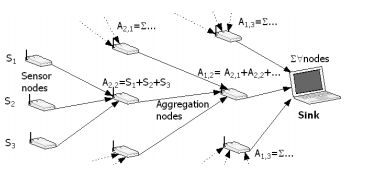
\includegraphics[width=0.5\textwidth]{/Users/rafaelremondes/UM/MEI/Thesis/Writing/Images/INA}
\caption{\label{fig:INAaggregation} Principle of in-network aggregation}
\end{figure}
An example of \text{in-network} aggregation in WSN is in  \cite{castelluccia2005efficient}. In this model, it is assumed that all nodes ate potential aggregators and that data gets aggregated as they propagate towards the sink. The aggregation is set as must being simple not involve any expensive or complex computation. The aggregation requires all sensors to send their data to the sink within the same sampling period so there is a need for a global so that all node can synchronize. Another study is in \cite{Girao2004c}, where a special kind of distributed aggregation is proposed, \textit{Concealed Data Aggregation}. This type of aggregation is defined as an approach than promises the combination os end-to-end security and \textit{in-network} aggregation. In \cite{chan2006secure} it is assumed a general multi-hop network with a set $S={s_1....s_n}$ of $n$ sensor nodes anda a single base station $R$. The aggregation is performed over an \textit{aggregation tree} which is the directed tree formed by the union of all the paths from the sensors nodes to the base station. Another WSN distributed aggregation scenario is presented in \cite{yu2009distributed}. The network model consist of a $n$ sensor nodes and one base station that is also called a sink. Each sensor node can send or receive data to or from all directions. It is assumed that all nodes have the same transmission range for simplicity. A node can either receive or send data at a time and it can receive a data packet correctly when it hears only this packet at that moment.


\section{Smart Metering Aggregation Model} 
There are two main architectures for smart metering considering data aggregation  are \textit{centralized} and \textit{distributed} or \textit{ decentralized}\cite{journals/spm/ErkinTLP13}. In \textit{centralized} fashion, the meters just sense the data, afterwards, it is sent to a central aggregator with higher computation power that holds a central database. In a \textit{decentralized} way, the aggregation role is distributed among several meters, not all of then. This type of aggregation is also called  \textit{in-network} aggregation \cite{Girao2004c}\cite{Castelluccia05efficientaggregation}. The aggregation node in this scheme communicate the calculated energy consumed to an appropriate party such as a energy producer. Typically, this communication occurs once per billable period \cite{journals/spm/ErkinTLP13}. As introduced before, the architecture chosen for this work is \textit{de-centralized} due to the nature of the aggregation algorithms.\\
In the literature, it is possible to find some particular studies. Keita Suzuki \textit{et al} \cite{DBLP:conf/isgteurope/SuzukiNYKMKA13}  presents a particular case in a office building in Japan(Heating ventilation and air conditioning facilitie,HVAC) where existis the need to aggregate power curtailments from hundred or thousands of distributed HVAC facilities. Several smart meters where placed, connected to a Gateway that receives the consumption data for daily or monthly billing.  The Gateways are connected to a central ADR, Aggregation Cloud, which aggregates all the consumption.\\
Another work using a \textit{de-centralized} way is in Rottondi \textit{et al}\cite{rottondi2012}.  The smart meters generate the energy consumption measurements, the Gateways securely aggregate the metering data and external parties access the aggregation results. Each meter is directly connected to a Gateway, receiving data from a limited number of meters. At regular time intervals, 15 min in this case, the meter generate a measurement and send it to the Gateway. The overall scheme is presented in \ref{fig:meterArchitecture}.
\begin{figure}[h]
\centering
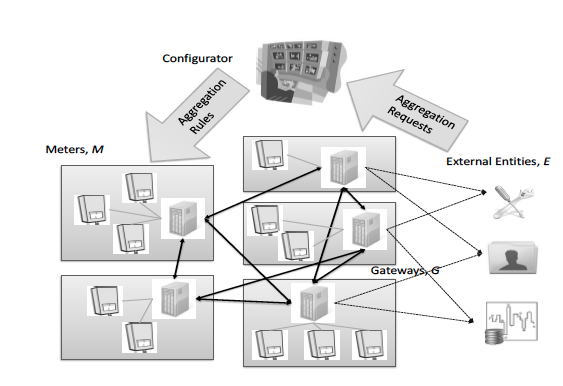
\includegraphics[width=0.5\textwidth]{/Users/rafaelremondes/UM/MEI/Thesis/Writing/Images/meterExample}
\caption{\label{fig:meterArchitecture} The functional nodes of the architecture}
\end{figure}

